\chapter{Creación de servicios de IoT en AWS y Azure}
Tanto Azure como AWS ofrecen servicios de mensajería entre dispositivos, como por ejemplo colas de mensajes. 

Ambos utilizan MQTT para la comunicación, aunque es posible en Azure utilizar su propio protocolo, pero no ofrece ventaja alguna sobre MQTT.

Vamos a demostrar las características de creación y administración de colas de mensajes y  los dispositivos que se conectan a ella.

Las ventajas de utilizar un servicio para este tipo de proyectos es el ahorro en costes de infraestructura y de seguridad que se tendría que realizar de forma manual, ya que habría que disponer de un servidor dedicado, exponerlo con seguridad a internet. Sin embargo, utilizando estos servicios nos tenemos que preocupar únicamente de desarrollar las aplicaciones, tampoco suponen un coste desorbitado, ya que para pocos dispositivos (50) es gratuito y a partir de ahí, el millón de mensajes entre dispositivos varía entre 0,7 y 1,5 dólares.

Además cabe mencionar la escalabilidad, que es la gran estrella de los servicios en la nube, poder escalar en caso de necesidad sin suponer una gran inversión ni tiempo.

\newpage
\section{Creación de servicios IoT en AWS}
En AWS tenemos que crear primero un Iot Center. AWS es sencillo de conectar, ya que al revés que Azure, en el cuál predomina su propio protocolo, se basa en el protocolo MQTT para transmitir los datos.
\begin{figure}[h]
	\centering
	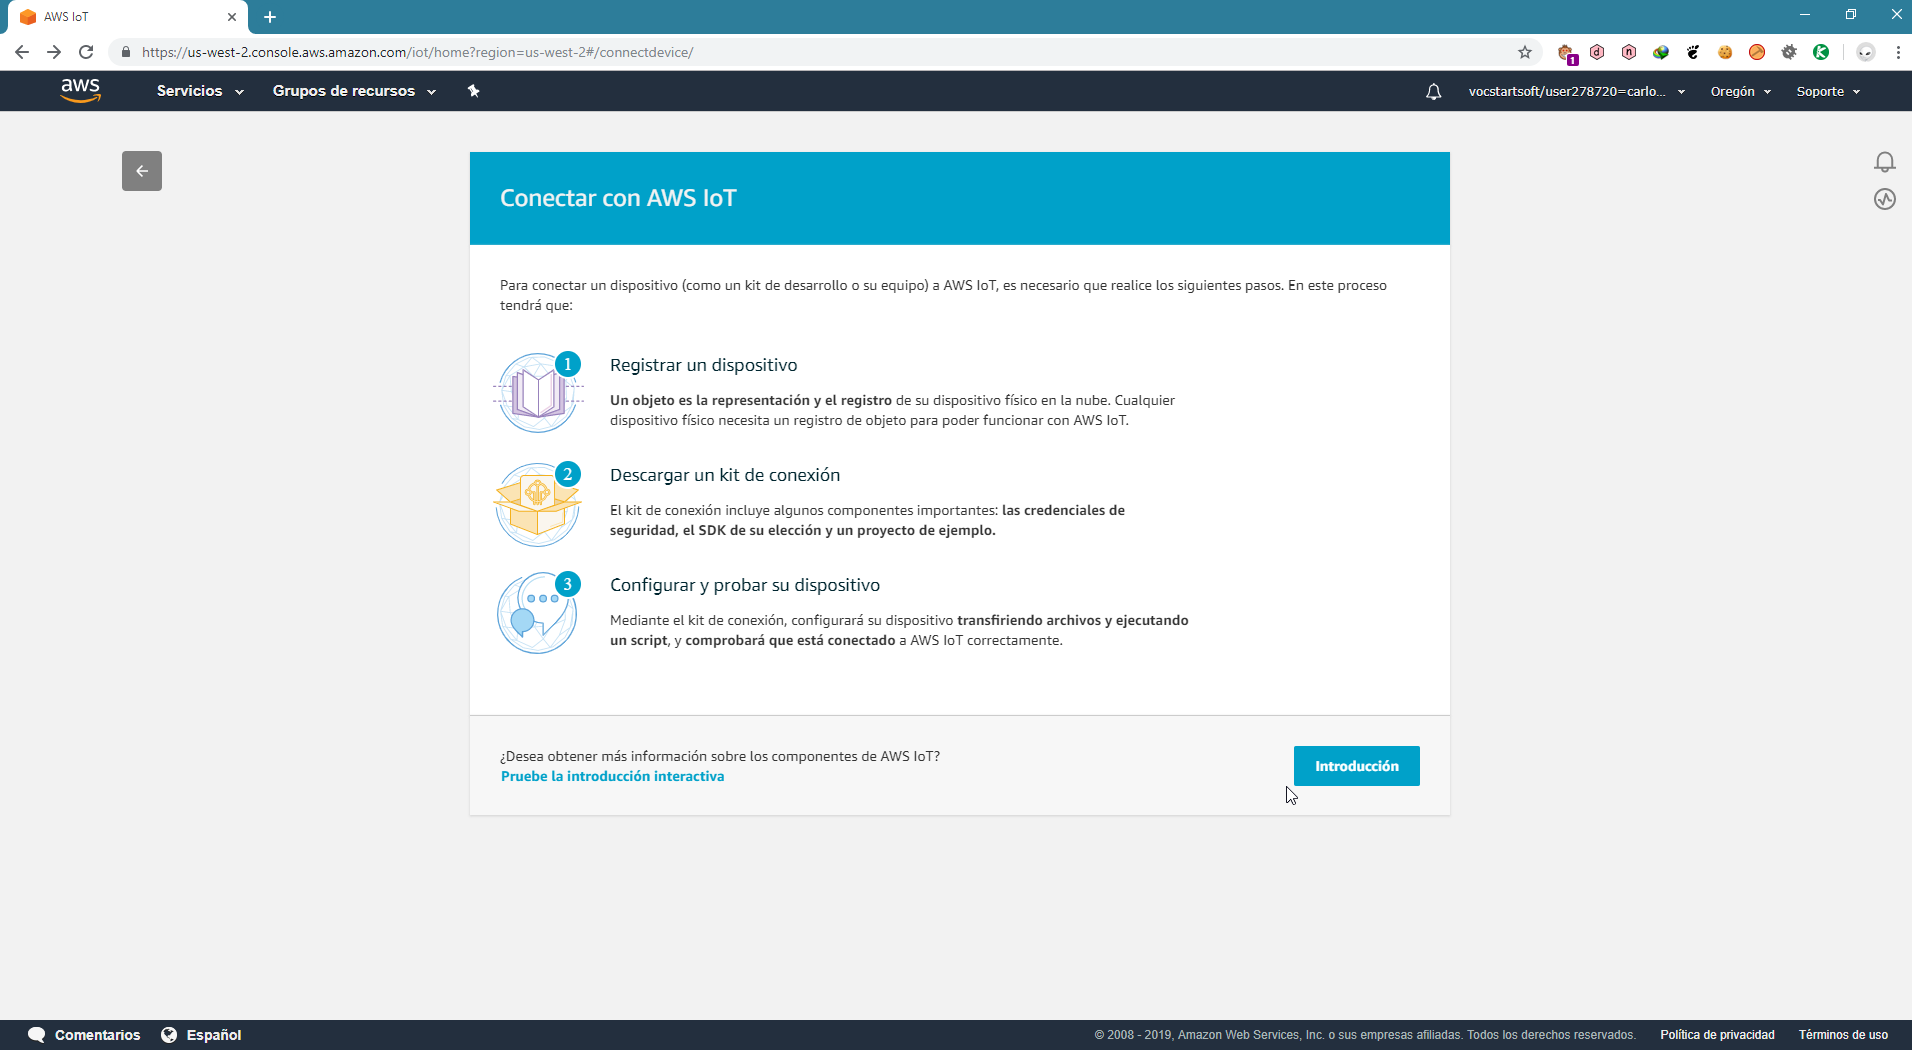
\includegraphics[scale=0.27]{iot_aws/creacion1.png}
	\caption{Creación del centro IOT}
	\label{AWSIOT1}
\end{figure}

Tras ver la introducción, se nos pide seleccionar el lenguaje a utilizar y el sistema operativo, para así poder descargar las herramientas que nos permitirán empezar a hablarnos con AWS a una cola MQTT.

\begin{figure}[h]
	\centering
	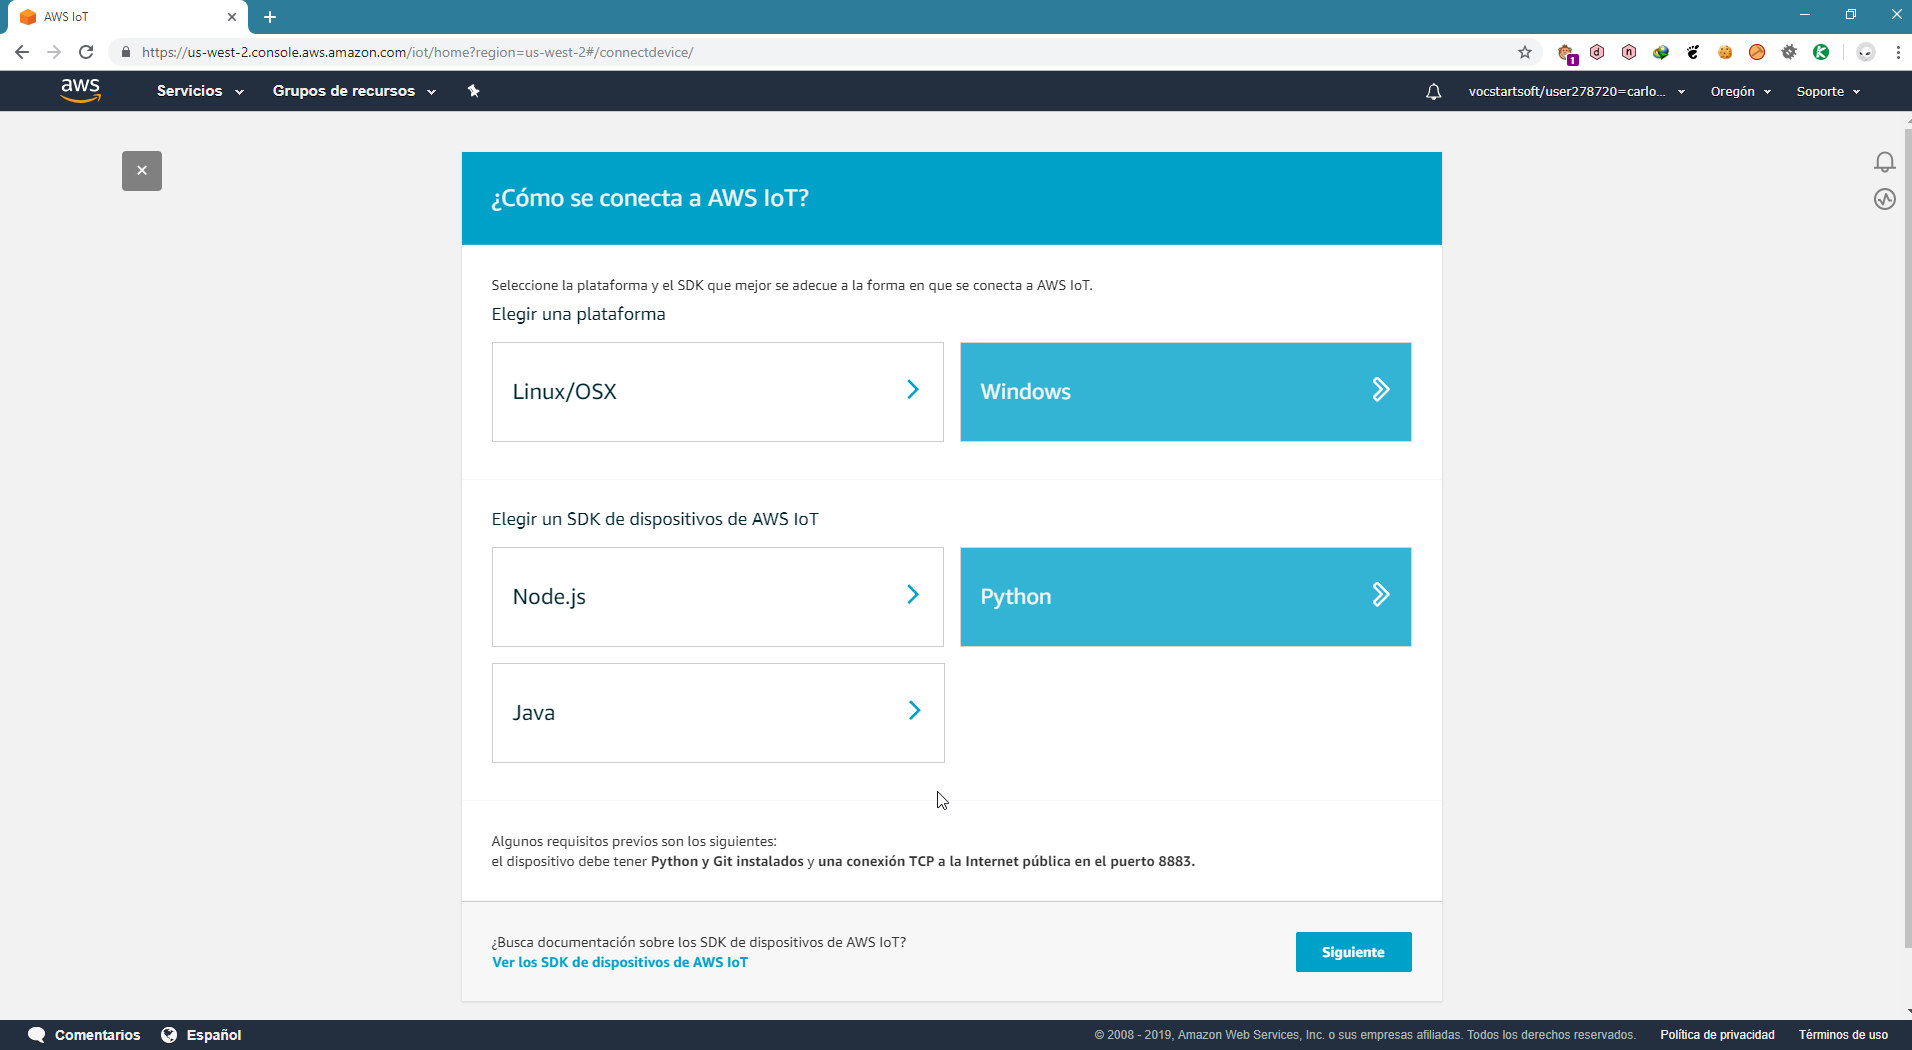
\includegraphics[scale=0.27]{iot_aws/creacion2.png}
	\caption{Selección del sistema operativo}
	\label{AWSIOT2}
\end{figure}

\newpage
Posteriormente tenemos que asignarle un nombre al objeto / dispositivo para poder reconocerlo en las métricas, ya que la autentificación, como se verá más adelante se realiza por medio de certificados.

\begin{figure}[h]
	\centering
	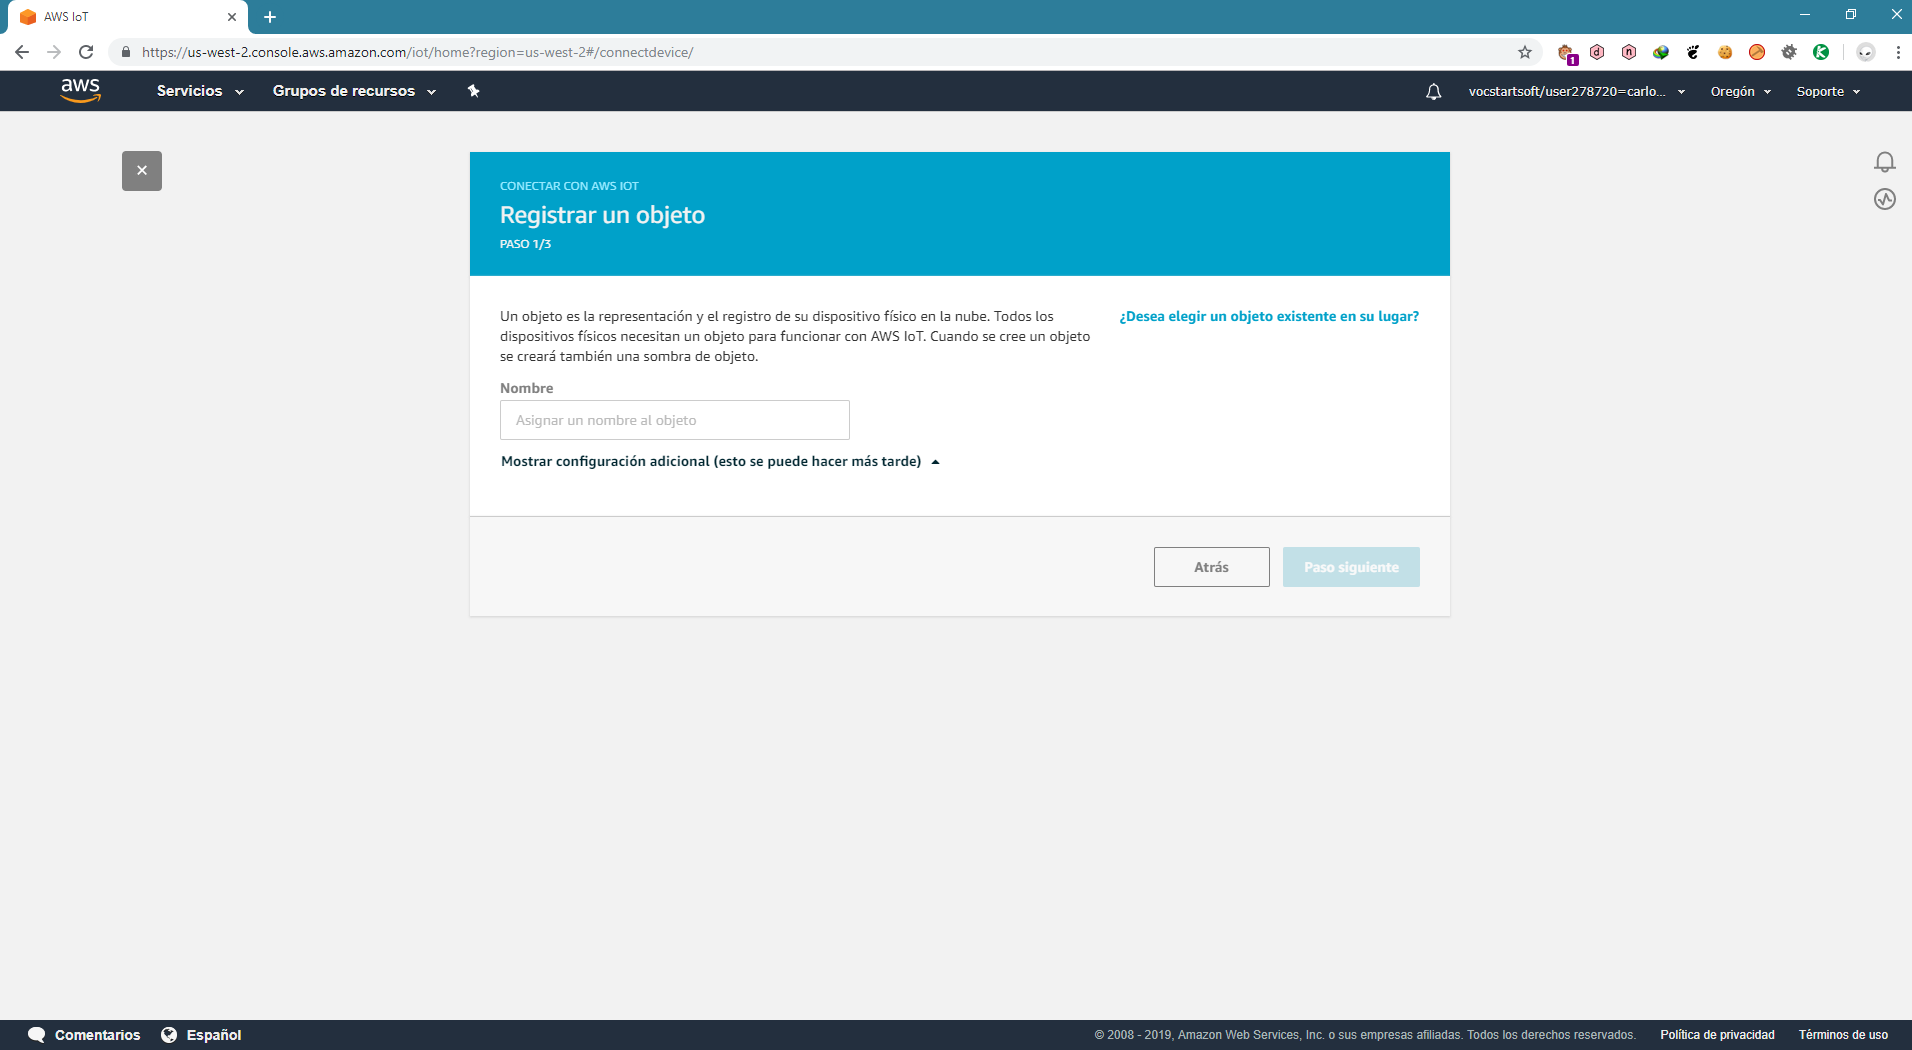
\includegraphics[scale=0.27]{iot_aws/creacion3.png}
	\caption{Selección del nombre del dispositivo}
	\label{AWSIOT3}
\end{figure}

Una vez creado el nombre, estamos listos para ejecutar los ejemplos que vienen con el kit de desarrollo, viene con todo lo necesario para empezar a comunicarnos con AWS, tanto los ejemplos como los certificados necesarios para autentificar el objeto anterior.

\begin{figure}[h]
	\centering
	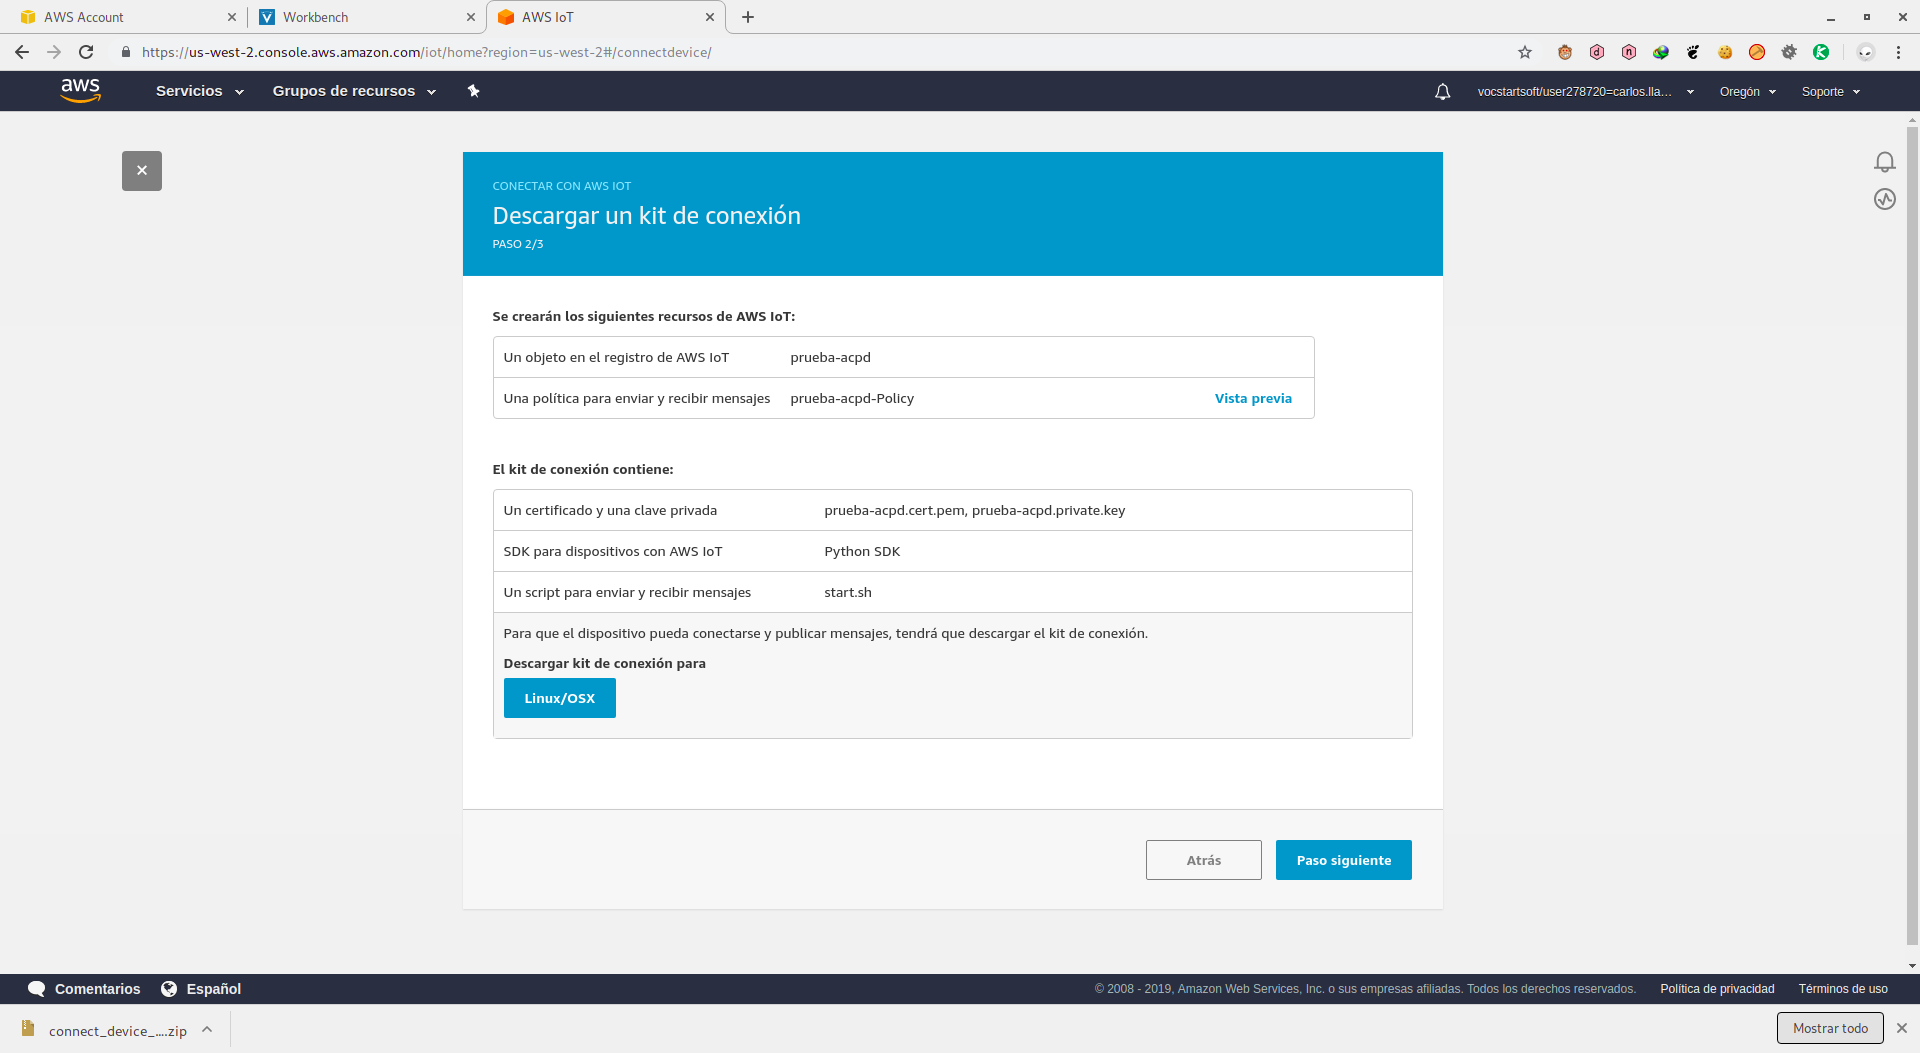
\includegraphics[scale=0.2]{iot_aws/creacion4.png}
	\caption{Descarga del kit de prueba}
	\label{AWSIOT4}
\end{figure}

\newpage
Posteriormente lo ejecutamos y empezaremos a ver como llegan mensajes y la aplicación de Amazon es capaz de leerla.

\begin{figure}[h]
	\centering
	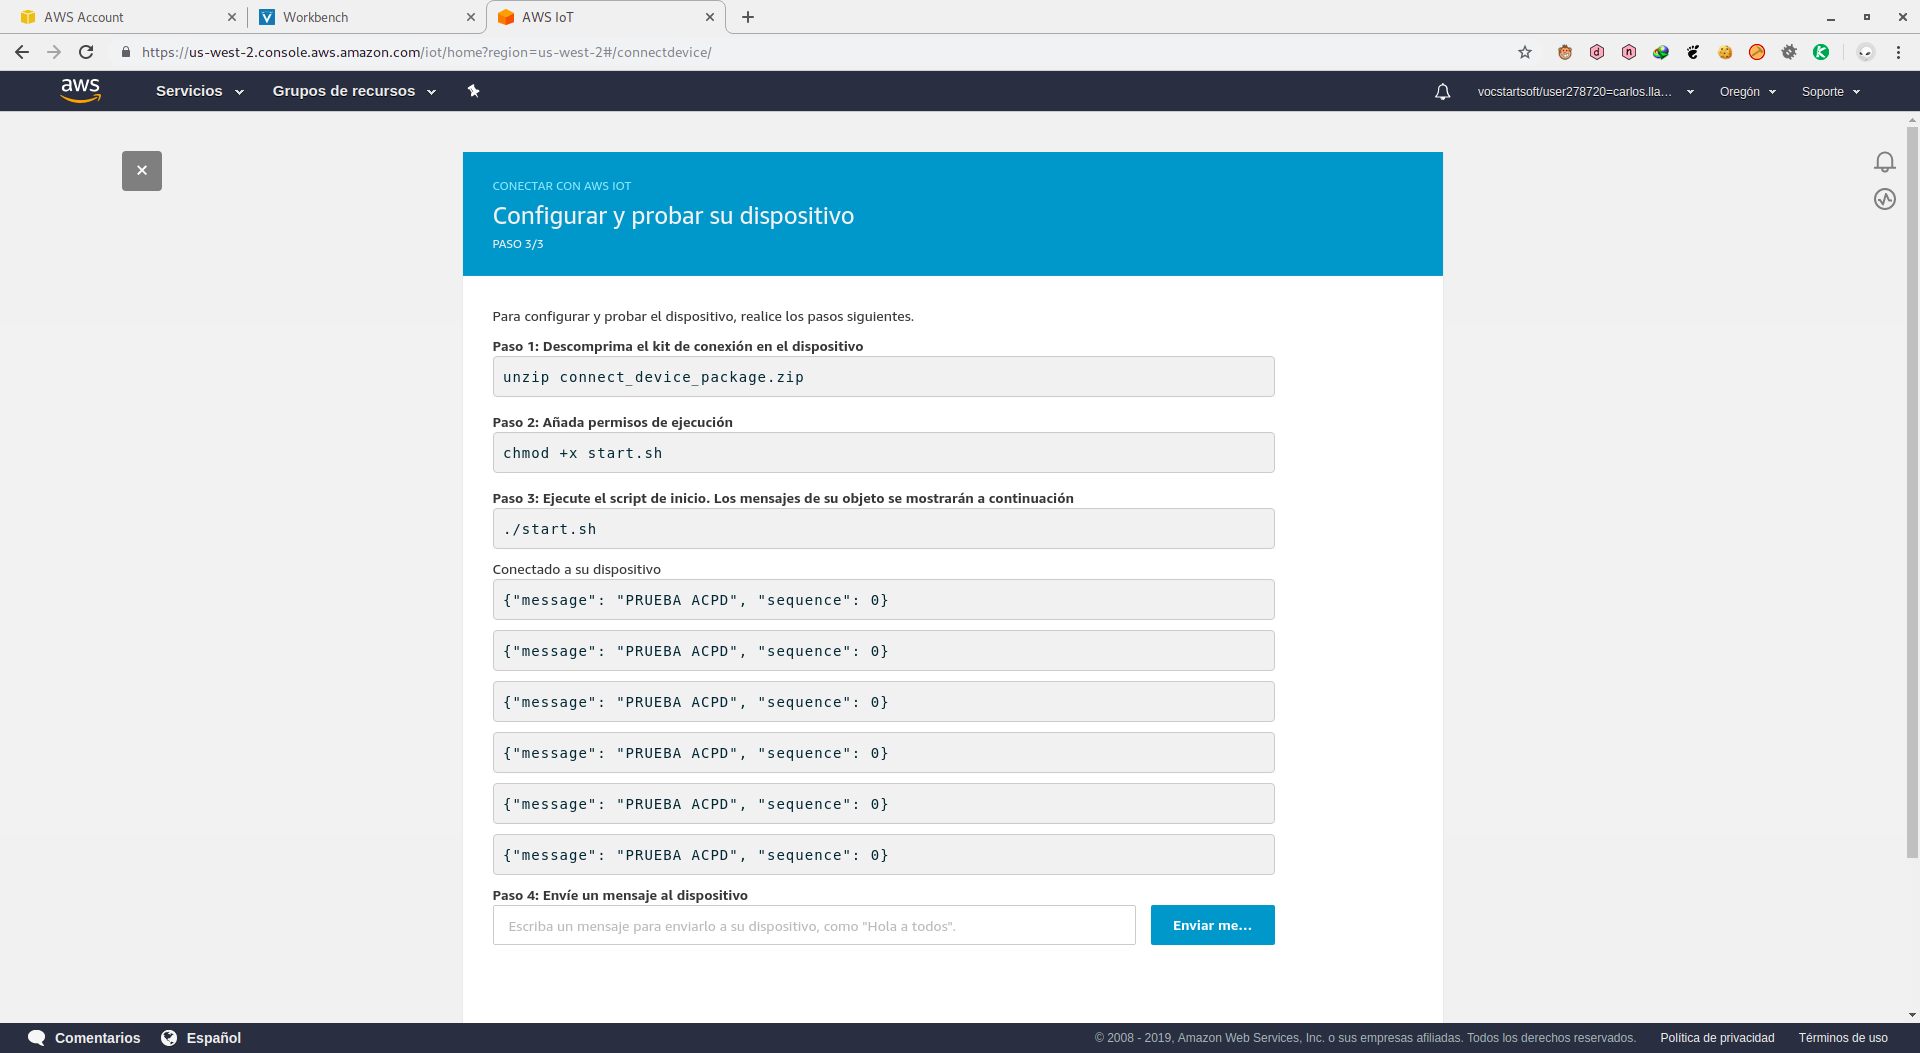
\includegraphics[scale=0.2]{iot_aws/creacion5.png}
	\caption{Prueba de ejecución}
	\label{AWSIOT5}
\end{figure}

Una vez llegado a este paso tenemos listo todo lo necesario para empezar a desarrollar nuestras aplicaciones sobre IoT.

También resulta interesante, añadir nuevos dispositivos / objetos, visualizar métricas de mensajes, modificar las políticas de seguridad de los dispositivos.

Para ello disponemos en el centro de IoT la sección de métricas:

\begin{figure}[h]
	\centering
	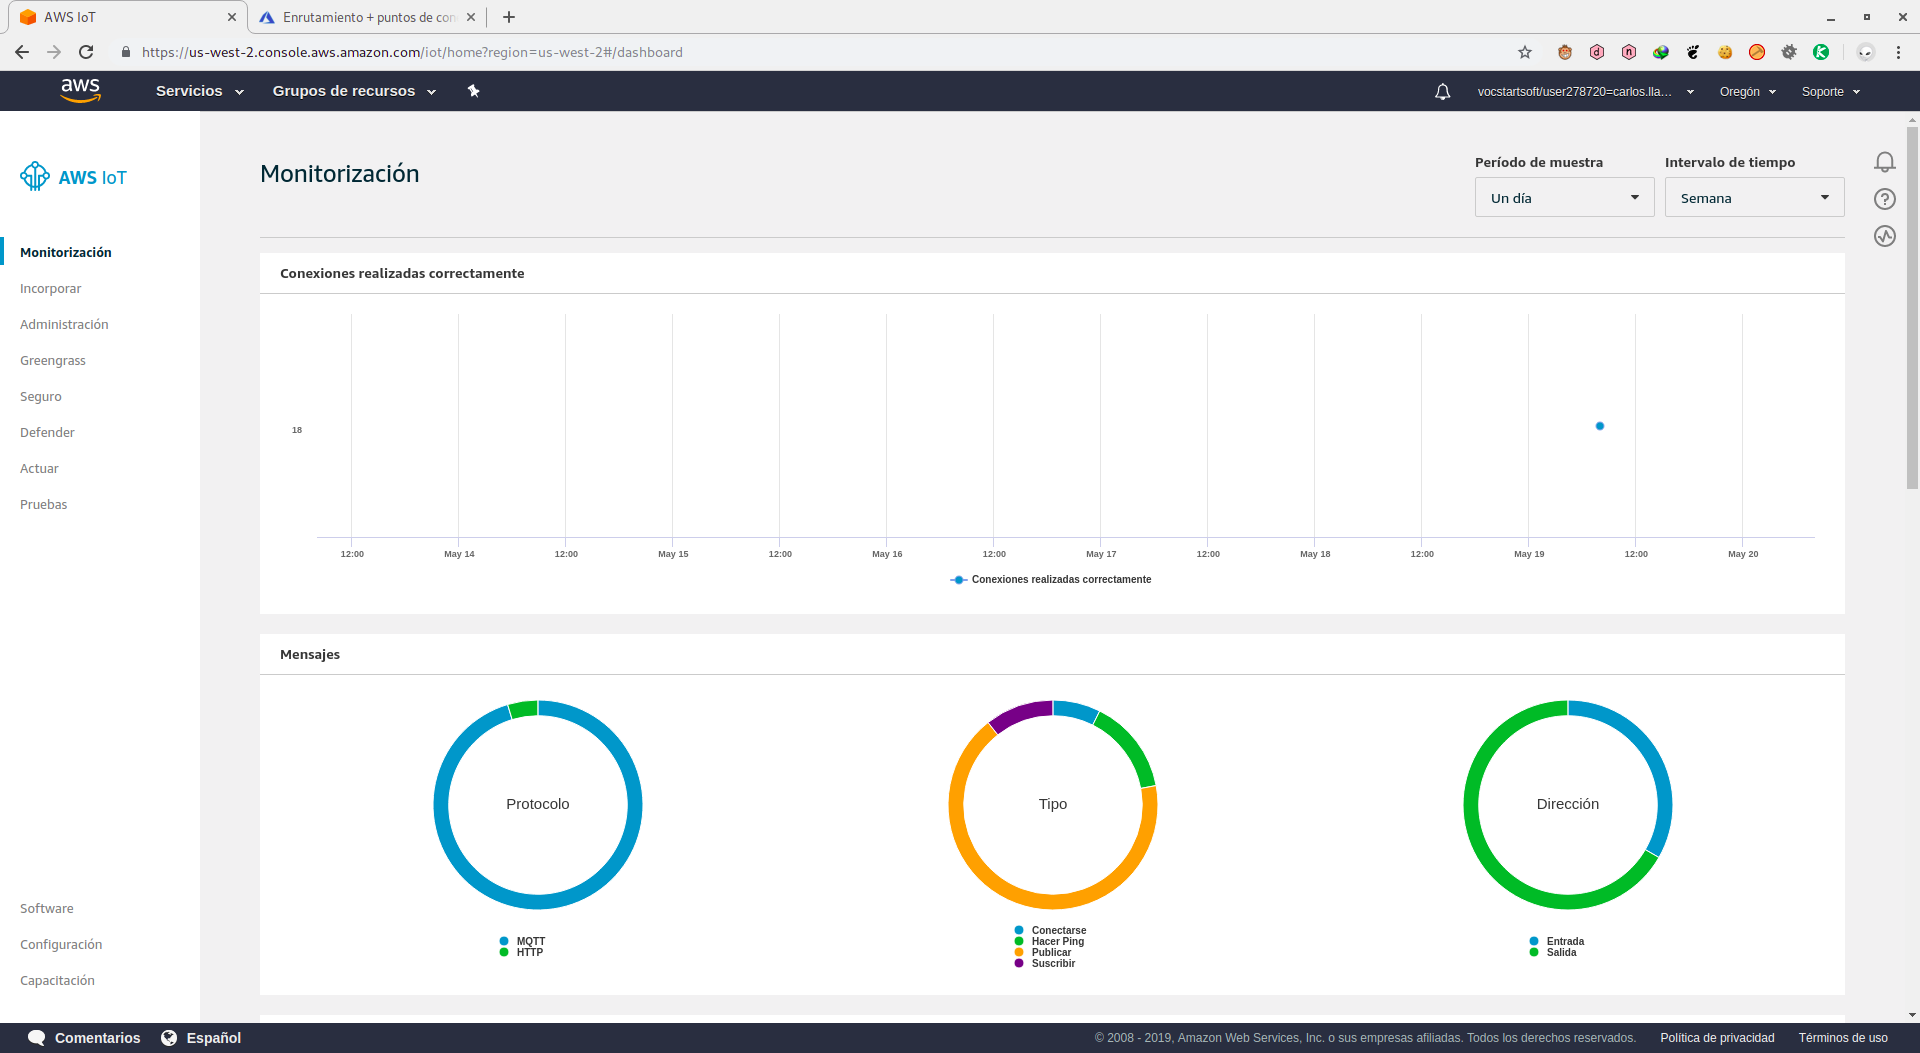
\includegraphics[scale=0.2]{iot_aws/centro.png}
	\caption{Visualización de las métricas}
	\label{AWSIOT6}
\end{figure}

\newpage
También disponemos una interfaz de gestión de dispositivos, donde podemos gestionar los parámetros de estos dispositivos:


\begin{figure}[h]
	\centering
	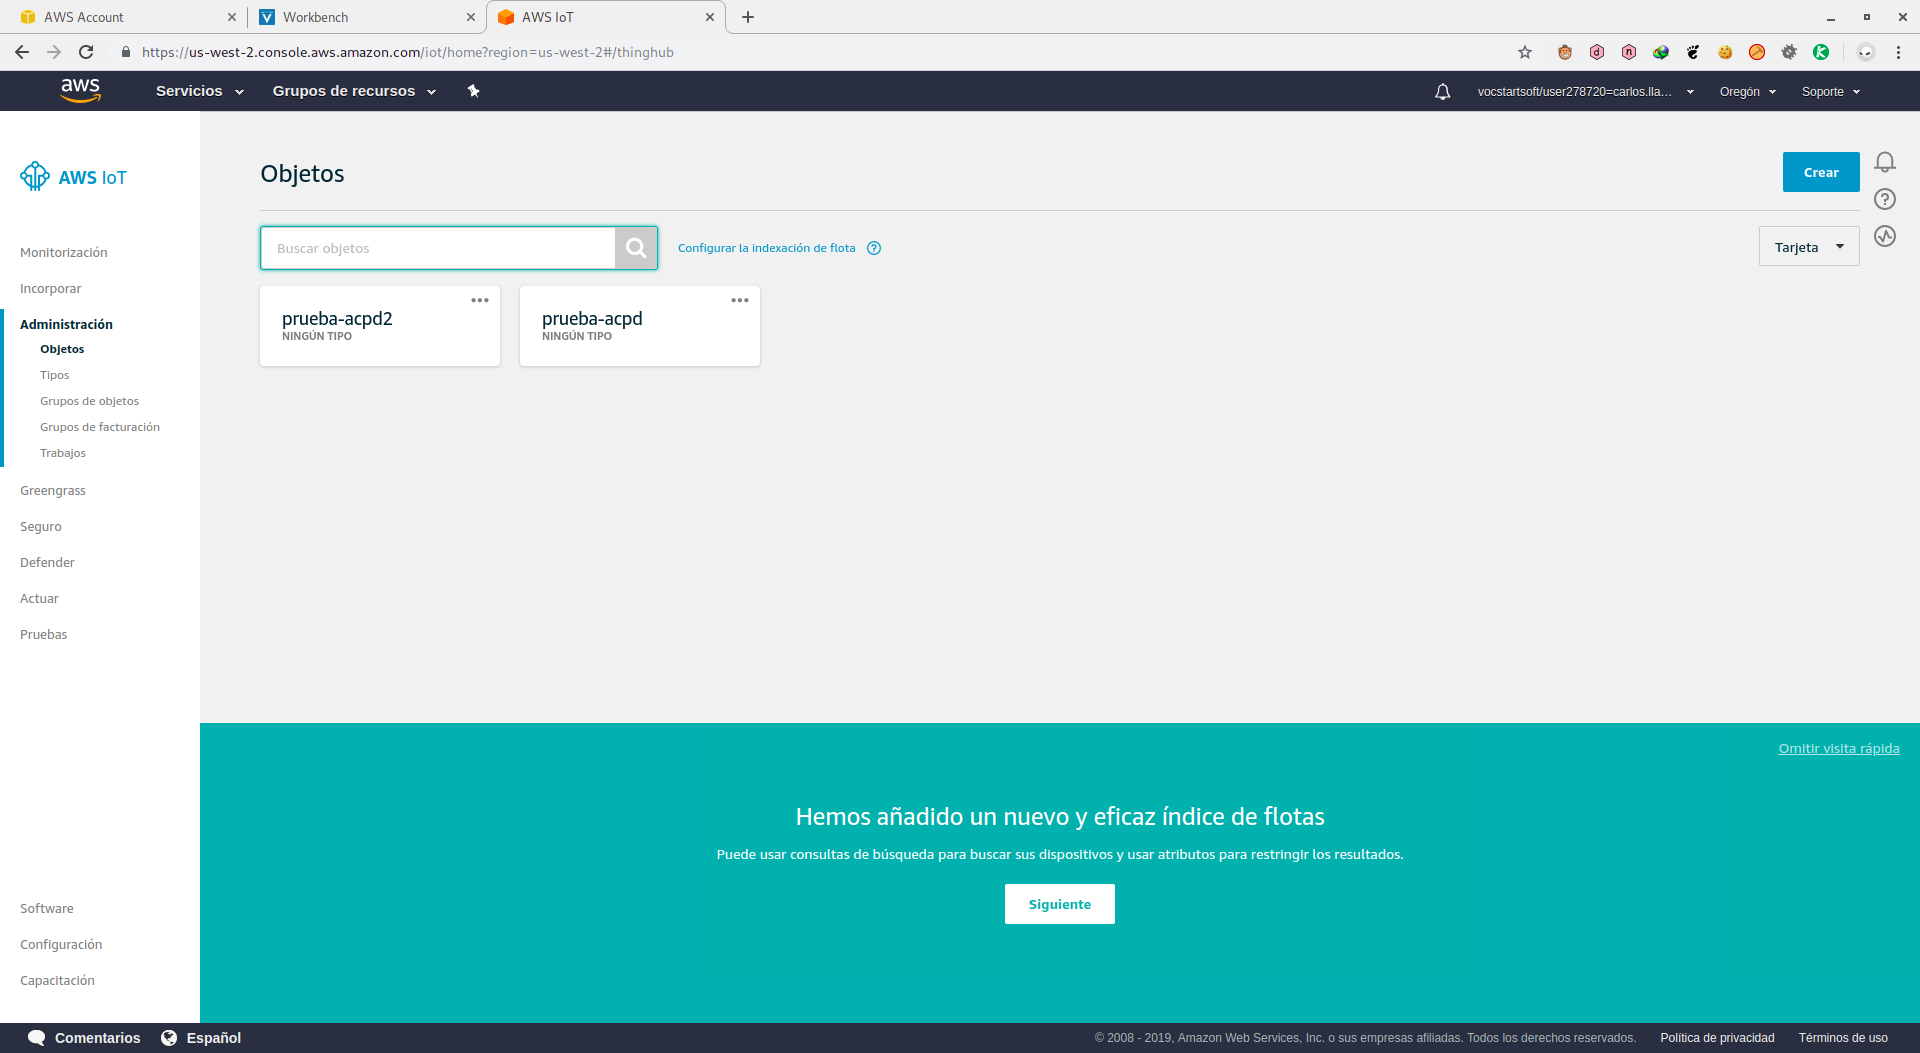
\includegraphics[scale=0.2]{iot_aws/dispositivos.png}
	\caption{Visualización del número de dispositivos}
	\label{AWSIOT7}
\end{figure}

\begin{figure}[h]
	\centering
	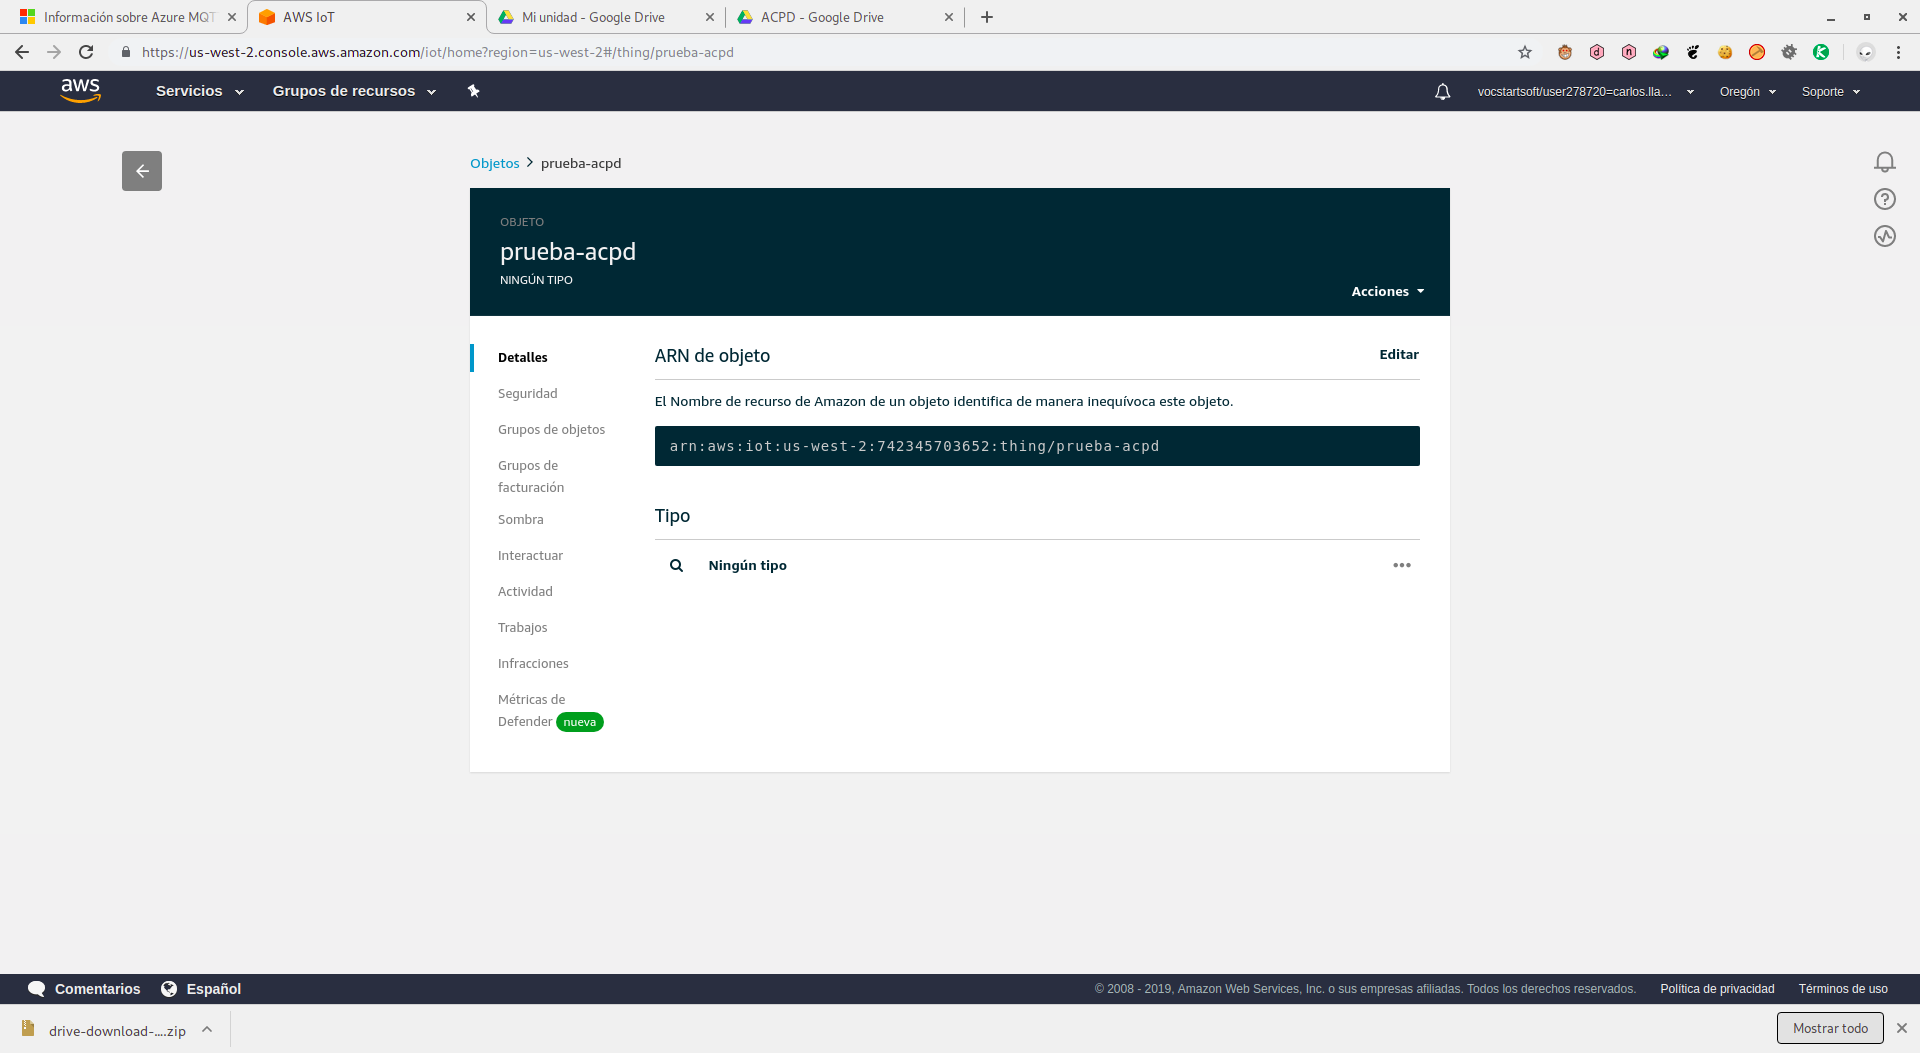
\includegraphics[scale=0.2]{iot_aws/dispositivos2.png}
	\caption{Gestión de un dispositivo}
	\label{AWSIOT8}
\end{figure}

\section{Creación de servicios IoT en Azure}
Ahora vamos a centrarnos en el servicio de Microsoft, la ventaja que tiene sobre AWS es la multiplataforma y la dedicación de Microsoft al IoT, ya que tiene distintas versiones de Windows adaptadas al IoT. Mientras que AWS soporta únicamente Java, Node.JS y Python, Azure lo expande con su plataforma estrella, .NET Core, a la que le está dando un gran empujón en los últimos años.

La ventaja de poder usar .NET Framework o .NET Core para desarrollar estas aplicaciones es la integración con el IDE Visual Studio, ya que prácticamente con 1 click podemos enviar la aplicación en la nube, como se vió en el apartado de desarrollo de servicios web.

Lo primero que hay que realizar en Azure es dar de alta un Centro de IoT o IoT Hub. Los grupos de recursos de Azure van enfocados a agrupar los recursos de cara a la facturación, en este caso al disponer de crédito gratuito podemos ignorarlo, con cuidado de no sobrepasar los límites.

\begin{figure}[h]
	\centering
	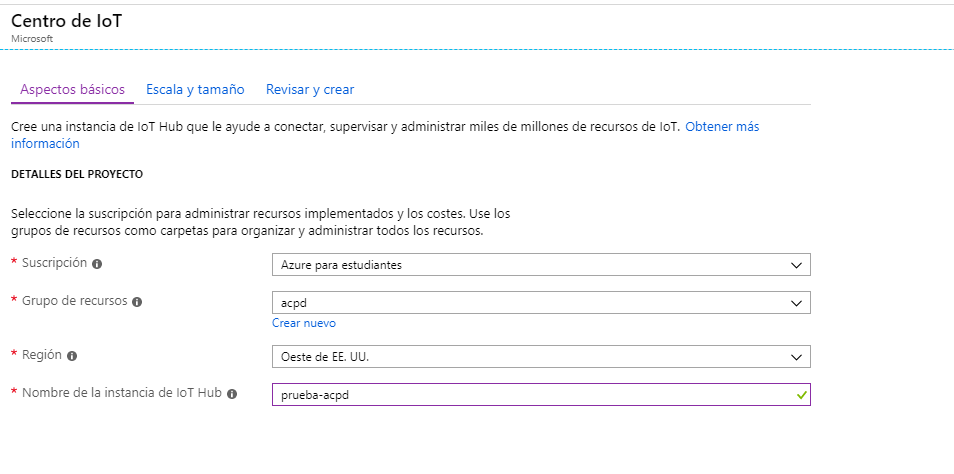
\includegraphics[scale=0.5]{iot_azure/primera.png}
	\caption{Creación de un centro IoT}
	\label{AZIOT1}
\end{figure}

Lo siguiente que se nos pide es la escala, a diferencia de AWS que no necesita escalar, si no que cobra por tramos de mensajes, Azure es necesario predefinir una escala, aunque no lleguemos a ella siempre se nos cobrará lo mismo. En este caso Azure tiene una versión gratuita para 8000 mensajes diarios.

\begin{figure}[h]
	\centering
	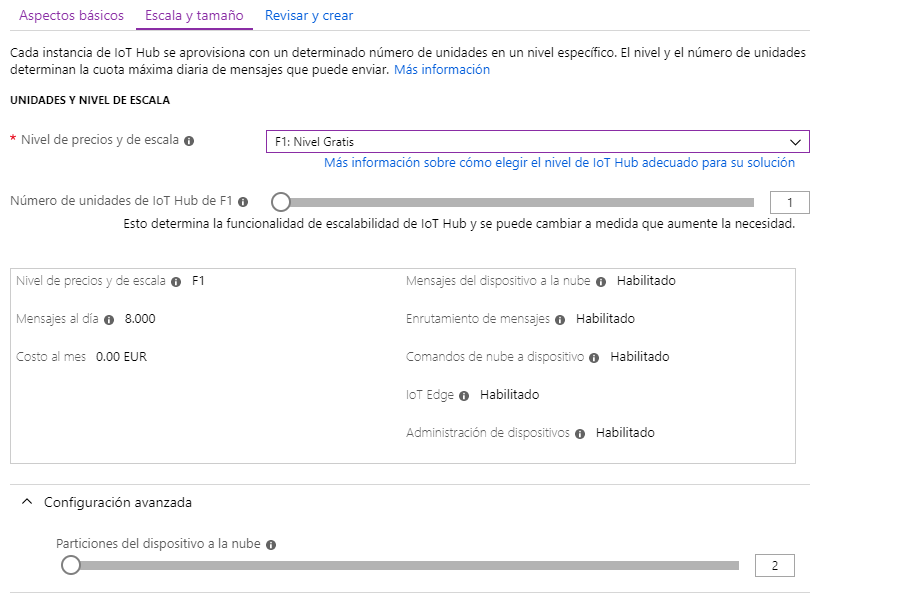
\includegraphics[scale=0.5]{iot_azure/escala.png}
	\caption{Selección de la escala}
	\label{AZIOT2}
\end{figure}

\newpage
Lo próximo que hay que realizar es añadir un dispositivo nuevo. A diferencia de AWS, Azure sí que te deja poner una clave en vez que utilizar certificados.

\begin{figure}[h]
	\centering
	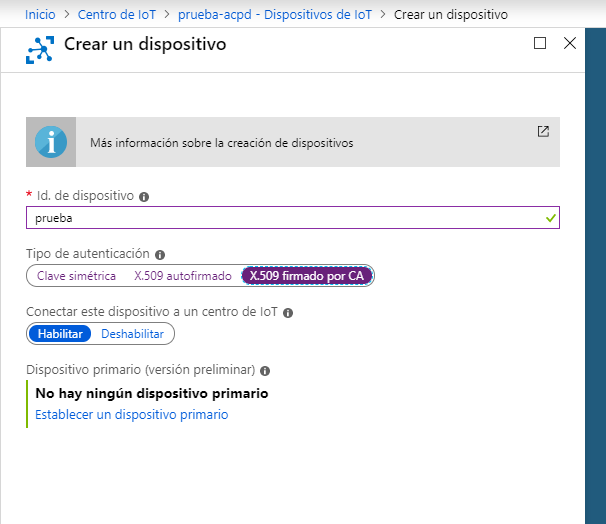
\includegraphics[scale=0.5]{iot_azure/dispositivo.png}
	\caption{Creación de dispositivo}
	\label{AZIOT3}
\end{figure}

Podemos ver los dispositivos en la lista de dispositivos.


\begin{figure}[h]
	\centering
	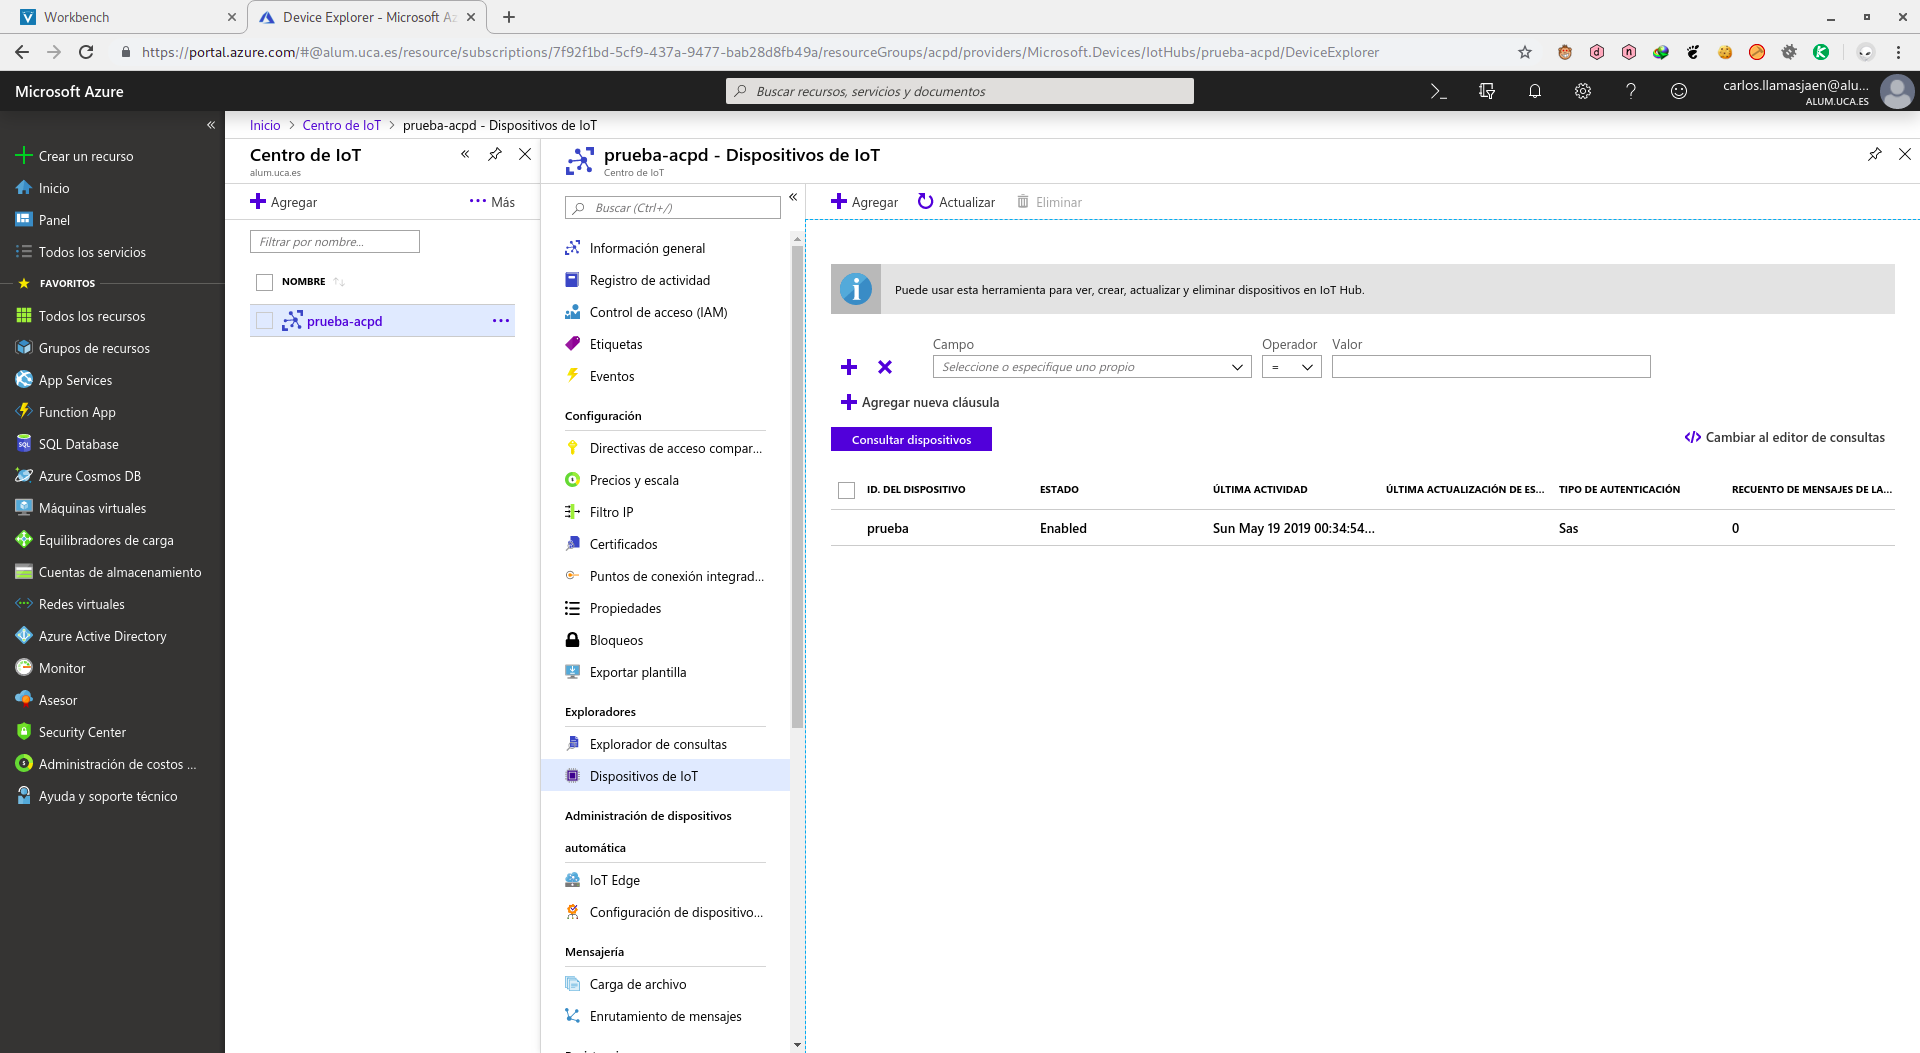
\includegraphics[scale=0.2]{iot_azure/dispositivos.png}
	\caption{Lista de dispositivo}
	\label{AZIOT4}
\end{figure}

\newpage
Una vez listo podemos volver al centro de IOT. Desde aquí podemos establecer políticas de seguridad, filtros, gestionar certificados, mirar métricas, eventos y gestionar la mensajería.

\begin{figure}[h]
	\centering
	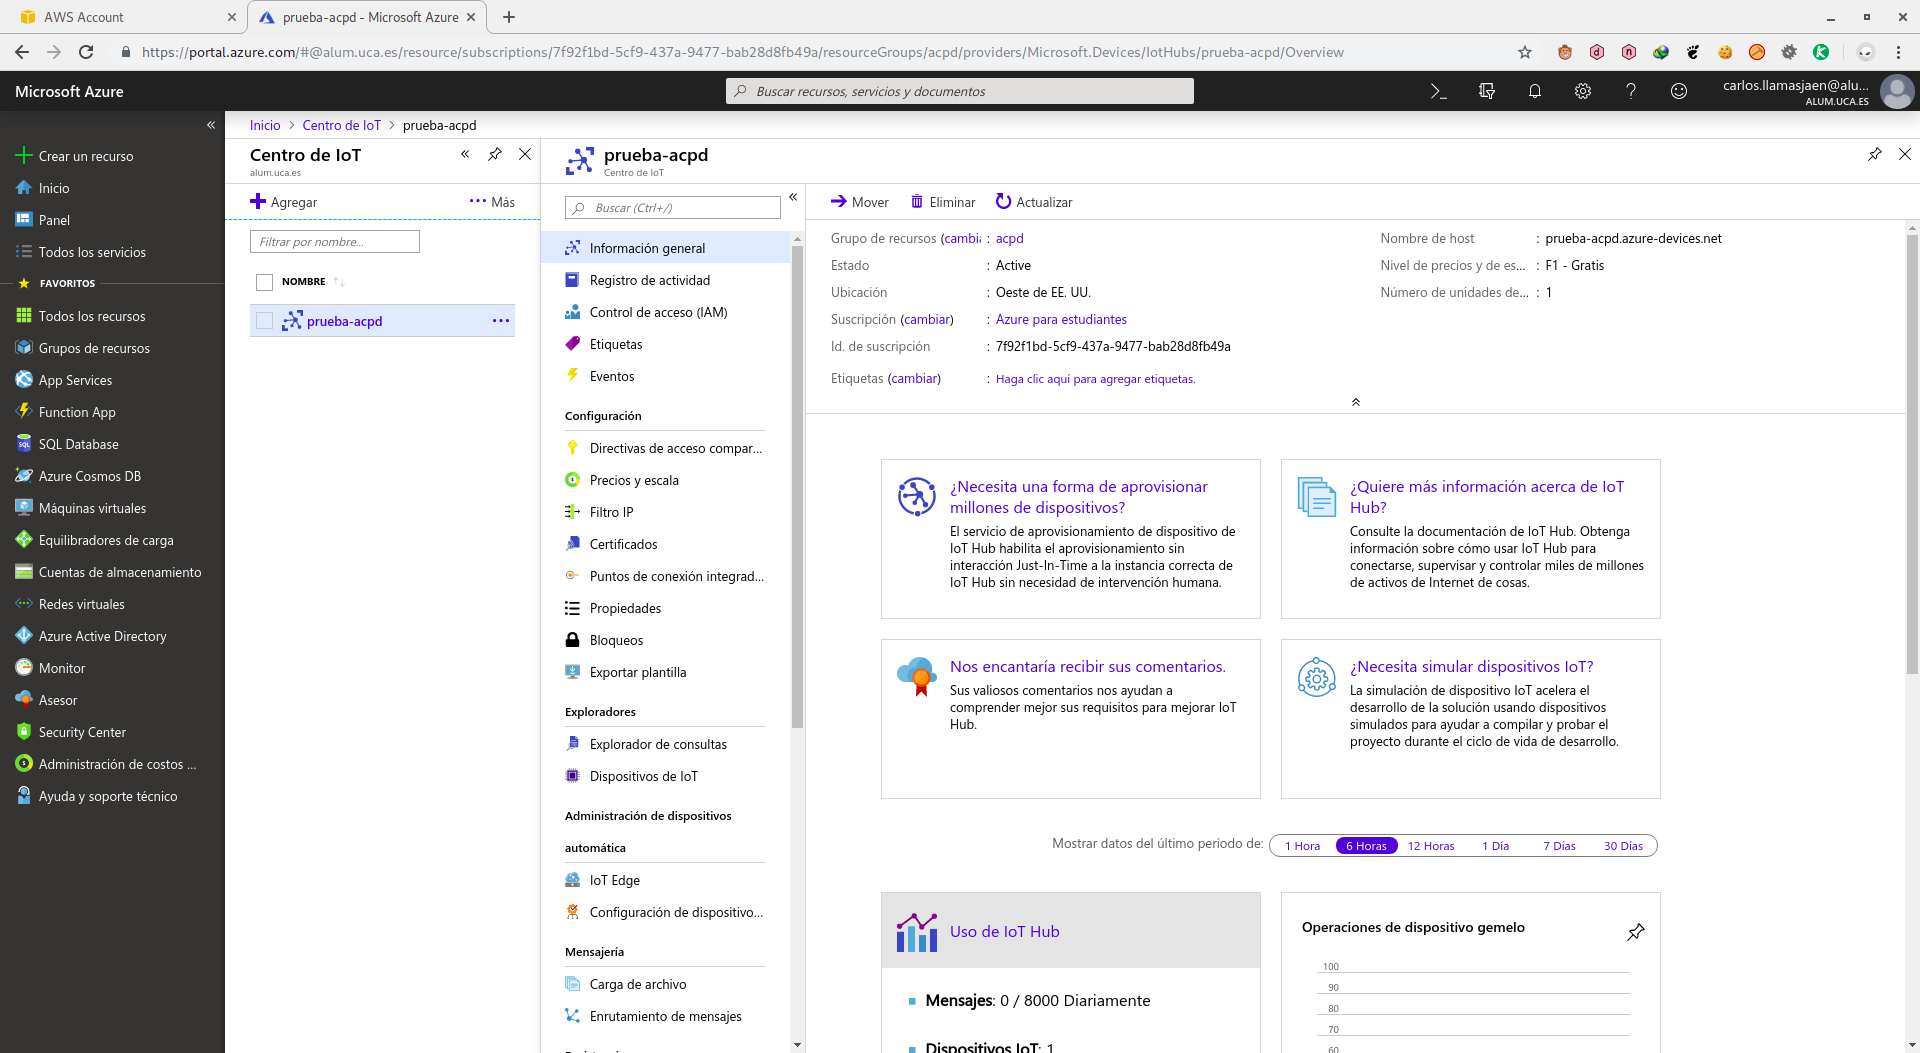
\includegraphics[scale=0.2]{iot_azure/centro.png}
	\caption{Centro de IoT}
	\label{AZIOT5}
\end{figure}

Pues con todo esto listo vamos a probar a ejecutar un ejemplo, para ello tenemos que crear otro dispositivo más y obtener las claves, es posible que haya que utilizar la CLI de Azure, que es de pago, ya que tiene que crear una pequeña cuenta de almacenamiento para poderla usar.


\begin{figure}[h]
	\centering
	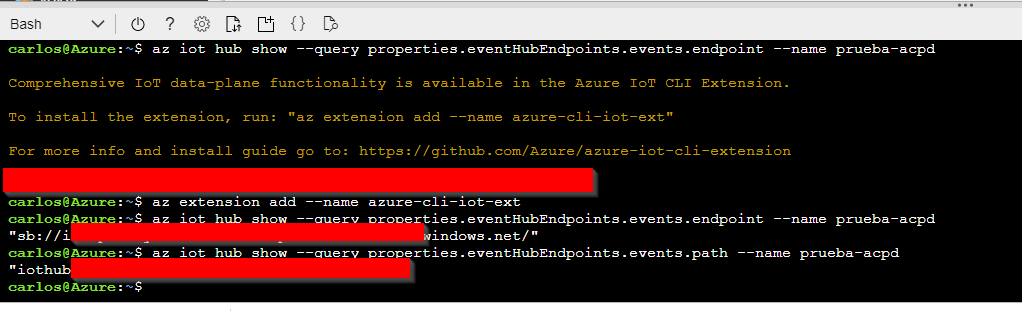
\includegraphics[scale=0.6]{iot_azure/azure_cli.png}
	\caption{Utilización de la Azure CLI para obtener las claves de los dispositivos.}
	\label{AZIOT6}
\end{figure}

\newpage

Una vez establecidas las claves, probamos un ejemplo que hay de IoT Hub, este ejemplo un publicador envía la temperatura de una sala y un suscriptor la recibe. En rojo aparece marcados los mensajes correspondientes que se envían desde el publicador y aparece en el suscriptor.

\begin{figure}[h]
	\centering
	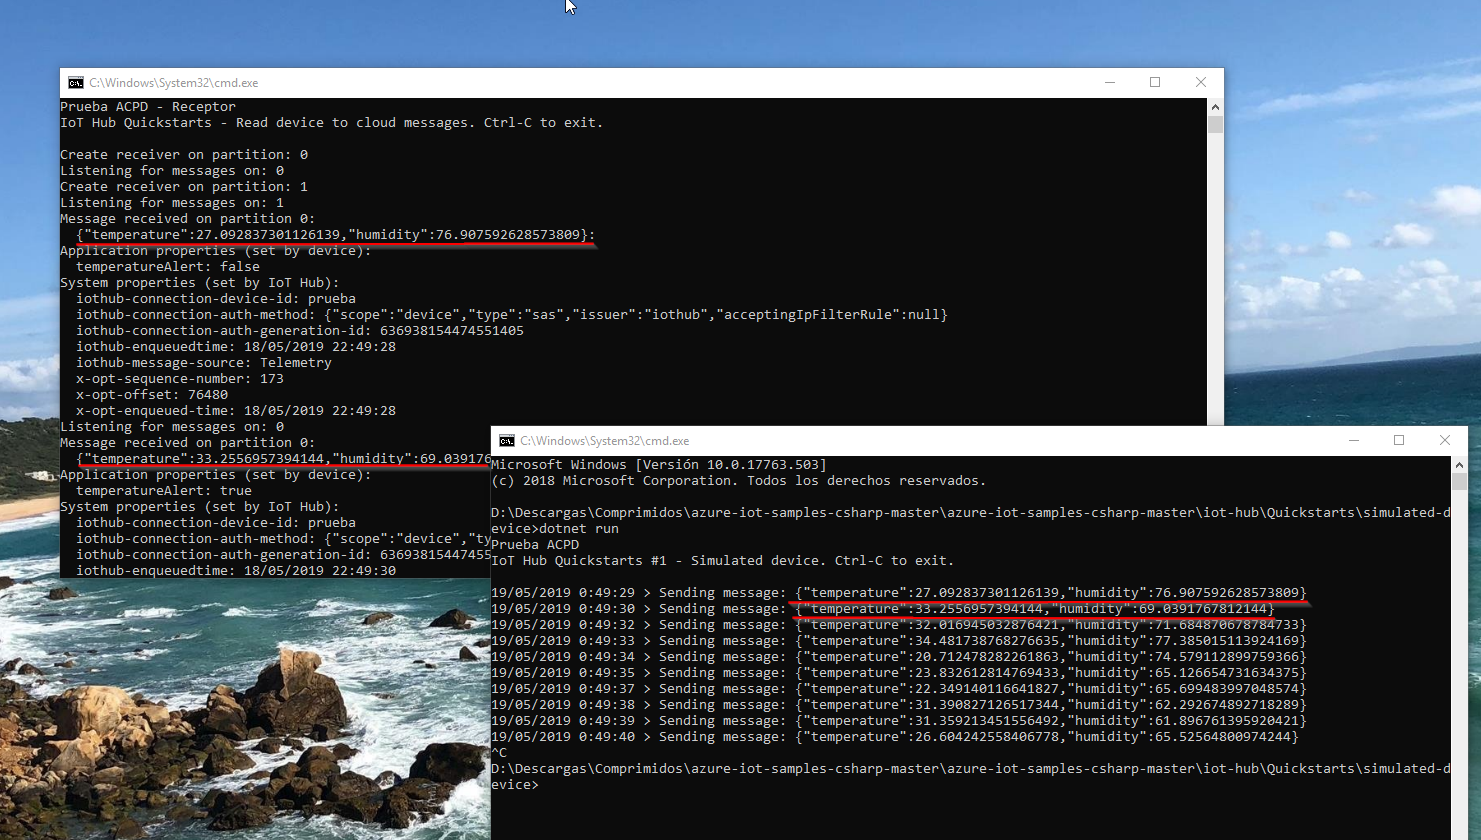
\includegraphics[scale=0.4]{iot_azure/mensajes.png}
	\caption{Ejemplo de IoT}
	\label{AZIOT7}
\end{figure}

